\chapter[Dietary gaps in sub-Saharan Africa: prevalence and implications for agricultural interventions]{Dietary gaps in sub-Saharan Africa: prevalence and implications for agricultural interventions}
\chaptermark{Dietary gaps in sub-Saharan Africa}
\label{cha:chapter6}
\vspace*{\fill}
This chapter is based on:
\\
\\
% Full citation of the published (or submitted/in review) article
% This refers to the article key in the refs.bib file.
Fraval, S., Hammond, J., Bogard, J. R., Ng'endo, M., van Etten, J., Herrero, M., Oosting, S. J., de Boer, I. J. M., Lannerstad, M., Teufel, N., Lamanna, C., Rosenstock, T. S., Pagella, T., Vanlauwe, B., Dontsop-Nguezet, P. M., Baines, D., Carpena, P., Njingulula, P., Okafor, C., Wichern, J., Ayantunde, A., Bosire, C., Chesterman, S., Kihoro, E., Rao, J., Skirrow, T., Steinke, J., Stirling, C. M., Yameogo, V., van Wijk, M. T. (submitted). \textit{Global Food Security}

\newpage

\section*{Abstract}
Efforts to estimate the prevalence of food insecurity and to understand its associations with rural livelihoods has been hampered by limitations in temporal and spatial representativeness. Food balance sheets provide scalable estimates of chronic and hidden hunger, but fail to represent food access, stability and their causal linkages. In contrast, rural household surveys represent detailed conditions for one or two points of time, but are influenced by survey timing and are often limited in geographical coverage. This study draws on a large sample of rural land-holding households in SSA (n = 6,353; 54\% of which were from semi-arid zones) to estimate the prevalence of dietary gaps and to understand their associations with rural livelihoods and food sourcing behaviour throughout the year. Dietary gaps were identified using diet diversity and food access indicators. Dietary diversity and channel of access (farm or purchased) were enumerated for the `flush' and `lean' periods and food security of access was enumerated for the lean period only -- making the results of this study independent of survey timing. The identified dietary gaps were then compared with quantified dietary adequacy ratios of subsistence households, and only included in further analysis if there was a statistically significant association. As many as 40\% of households were classified as severely food insecure (in terms of food access) in the lean period. Prevalence of micronutrient dietary gaps were high, with 68\% lacking daily calcium sources, 38\% lacking daily sources of iron, 37\% lacking daily sources of thiamine, 51\% lacking daily sources of riboflavin, 44\% lacking daily sources of niacin, 35\% lacked a source of vitamin B6 and 65\% lacking daily sources of vitamin B12. Vulnerability to dietary gaps differed by household composition and agricultural livelihood characteristics. Market participation, livestock product diversity, crop production diversity, gross income and off-farm income were all positively associated with food security of access and micronutrient access. These associations differed between agro-ecological zones and were predicted to have a limited impact on dietary gaps. Households with a livestock component to their farm consumed more milk, meat and eggs (sources of calcium, riboflavin and vitamin B12). Dairy, fruit and vitamin A-rich produce were  predominantly accessed through the farm channel. Households with a livestock component to their farm had a lower prevalence of severe food insecurity and gaps in micronutrient sources.

These findings have implications for the development of nutrition-sensitive and nutrition-specific interventions. Interventions need to be tailored to agroecological zone, household composition, scale of operation and production mix. Increasing income will not necessarily result in improved diet diversity or healthy dietary choices. Interventions focused on income generation should monitor and promote crop and livestock production diversity and provide nutrition education. Our analysis suggests that it is unrealistic or may even be counterproductive to try and shift overall diet diversity substantially, rather it is more useful to target individual food groups that will benefit human nutrition.

\newpage

\section{Introduction}

Almost one in four people in sub-Saharan Africa (SSA) were estimated to be undernourished in 2017, representing about one-third of the 821 million people suffering from chronic hunger globally (\citealp{FAO2018}). In addition to a high prevalence of chronic hunger in SSA, many more people suffer from micronutrient deficiencies (\citealp{Harika2017, Kumssa2015, Joy2014}). These deficiencies increasingly co-exist with instances of obesity within the same communities -- forming a triple burden on human health and society (\citealp{May2018}). Malnutrition is now the greatest risk factor driving a rising global noncommunicable  disease burden (\citealp{GBD2016RiskFactorsCollaborators2017}), having direct implications for child growth failure, neonatal disorders, immune function, cognitive function, diabetes, heart disease and cancer (\citealp{James2018}; \citealp{Prentice2018}; \citealp{DePee2017}; \citealp{Pisa2017}; \citealp{Akombi2017}; \citealp{Micha2015}). These burdens will only intensify as rural and urban populations grow, diets change and wealth is further concentrated (\citealp{FAO2018}; \citealp{Popkin2014}).

The majority of the food in SSA is produced by smallholder farmers (\citealp{Herrero2017}) while they are the most vulnerable to food insecurity and poverty (\citealp{Fanzo2018}; \citealp{Sibhatu2017}). Hence, smallholder farmers are a crucial entry point for agricultural orientated interventions to improve food and nutrition security. A substantial number of observational studies have assessed the linkages between agriculture and nutrition in the past three years (e.g. \citealp{Ruel2018}; \citealp{Gillespie2017}). Despite progress in the analysis of existing observational data and ex-post evaluation of nutrition-sensitive interventions, much remains to be understood with respect to the pathways of intervention to improved food and nutrition security of rural households (\citealp{Mary2018}).

The causal pathways from intervention to food and nutrition security outcomes are not straightforward (\citealp{Carletto2017}). An important question, not yet answered by the existing literature (e.g. \citealp{Ruel2018}; \citealp{Gillespie2017}) relates to how market participation mediates food and nutrition security in rural communities -- especially access to and consumption of diverse diets. Farmers have two ways to obtain their food: 1) growing food crops and/or rearing livestock to consume the products, or 2) selling these products and use the income to buy food for their own consumption. Whether production-based or income-based channels are more important for food and nutrition security is a question without a straightforward answer. For example, increased incomes and energy availability are necessary for alleviating undernourishment but are not sufficient for addressing chronic or hidden hunger (\citealp{Godecke2018}; \citealp{Schipanski2016}; \citealp{McDermott2015}; \citealp{Hoddinott2012}). These causal pathways need to be considered in targeting, designing and implementing nutrition-sensitive interventions of agricultural production systems and value-chains.

Evaluating food access and micro-nutrient deficiencies has traditionally been time-consuming and invasive. More recently, however, proxies have been introduced to enable wide-scale monitoring and evaluation. Food security of access scales and diet diversity scores (to a greater extent) have been favourably assessed as proxies for nutrient adequacy (\citealp{Lachat2017}; \citealp{Steyn2006}; \citealp{Torheim2004}) diet quality (\citealp{Savy2005}) and child growth/stunting (\citealp{Rah2010}; \citealp{Saha2009}; \citealp{Arimond2004}). The development of these time-efficient metrics has allowed for food and nutrition security indicators to be incorporate into large-scale, multi-purpose farm household surveys. Despite this progress, complications arise when relating farm information and nutrition information: there is a systematic mismatch of time scales. Food and nutrition security is typically assessed over short time scales (e.g. 24h or weekly recalls) whereas farm production and consumption of agricultural produce are typically estimated at annual or seasonal time scales (\citealp{Herrero2007}). Using the annual timescales commonly found in agricultural surveys can create problems because diets of rural households are often highly variable throughout the year (\citealp{Sibhatu2017}). For instance, diets in the period after crop harvest are substantially different from the most difficult period of the year. This variability in diet means that survey timing can significantly influence the dietary results obtained in the survey. This means that from a nutrition perspective, surveys need to be executed throughout the year to characterise that temporal variation, while agricultural surveys are usually only executed only once or twice in a year.

This present study seeks to combine diet diversity and food (in)security indicators with household-farm characteristics to estimate prevalence of dietary gaps and to understand their associations with rural livelihoods and food sourcing behaviour throughout the year. Agricultural systems in SSA are diverse and dynamic, and agro-ecological conditions drive their occurrence (e.g. \citealp{Garrity2012}). The amount and timing of rainfall determine which crops can be grown and when they can be harvested, thereby affecting the availability of food items throughout the year. The agro-ecological conditions also drive the occurrence of livestock systems, with (agro-)pastoral systems in dry areas, and mixed crop-livestock systems in higher rainfall zones. We quantify how farming system characteristics (with a focus on livestock holdings e.g. \citealp{Headey2018} and crop production diversity e.g. \citealp{Jones2016}) shape the different pathways to food security of access, more diverse diets and access to micronutrients. We do so, by modifying existing diet diversity and food (in)security indicators to 1) provide an overview of food security across the year -- independent of survey timing, and 2) identify the channel of food access (e.g. own-farm or purchased). For this purpose, we use the food security indicators included in the `rural household multiple indicator survey' (RHOMIS) initiative (\citealp{Hammond2017225}), with data collected from almost 8000 households in eight different countries in sub-Saharan Africa.

\section{Methods}

\subsection{Household data}

This study draws on responses from 7,708 rural land-holding households in SSA. Interviews were conducted through twelve projects operating across eight countries between 2016 and 2018 (Appendix Table \ref{tab:C_2} provides a summary of sample size by project and country). For the purpose of this meta-analysis, we filtered the database based on data quality criteria, which resulted in 1,355 observations being removed (Appendix Table \ref{tab:C_2} summarises thresholds for excluding observations).

The `rural household multi-indicator survey' (RHOMIS) was utilised for data collection in all projects, eliciting information about the household composition, farm characteristics, diet diversity and food (in)security of access. The survey is designed to minimise the time burden on the interviewee, to maximise the reliability of responses, and to improve consistency between different studies (described further in \citealp{Hammond2017225}). Households were sampled using a multi-stage clustered design with random selection of villages and households. The sampling of each study was designed to be representative of the rural land-holding population in a given location, except for one study in Tanzania where livestock holders were exclusively targeted (14\% of observations in this study).

We adapted existing diet diversity and food (in)security indicators for the purpose of this study. First, our Modified Household Diet Diversity (MHDD) indicator was based on the `minimum diet diversity for women' (MDD-W) indicator, which is based on a count of 10 food categories (\citealp{FAO2016}). The modification to the MDD-W indicator allowed households to recall the frequency of access for each food category in the best and worst month (referred to as `flush' and `lean' period herein) rather than 24-hour recall across multiple visits in a year. As an extension of diet diversity indicators, we also asked households to recall the channel of access for each food category -- farm, purchased or free/traded. Second, the `household food security of access prevalence' (HFIAP) indicator is based on a series of nine questions of increasing severity, from worry about food availability to missing an entire day of food due to availability (questions provided in Appendix Table \ref{tab:C_10}; \citealp{Coates2007}). Severe food insecurity (of access) is defined as regularly eating smaller meals than desired, regularly eating fewer meals than desired or worse. Our `modified household food insecurity of access prevalence' (MHFIAP) indicator recorded conditions in the worst month experienced (`lean' period) by the household during the previous 12 months (a modification of the 24-hour recall period recommended in the `Food And Nutrition Technical Assistance' (FANTA) guidelines; \citealp{Coates2007}). The modifications to the recall period were made so that indicator results would be independent of survey timing and provide greater temporal coverage, rather than providing a snapshot of one or two days.

Our analysis also incorporated demographic, agro-ecological, farm, and economic metrics. Adult equivalents were calculated as the ratio of energy requirements for an age and gender class relative to the average energy requirement of adult males and females between 25 and 50 (2500 kcal; following \citealp{ClaroRafael2010} and using energy requirements from \citealp{FoodandAgricuturalOrganization2001}). Agro-ecological zone (AEZ) was extracted from the \citet{Choice2015} AEZ-16 spatial layer based on global-positioning system (GPS) points. Market participation was calculated as the proportion of crop and livestock calories sold. Tropical Livestock Units (TLUs) were calculated using conversion factors provided by \citet{Njuki2011a}. The `progress out of poverty index' (PPI) was calculated using 10 questions on household characteristics (e.g. housing structure, asset ownership, school attendance) that are correlated with country specific poverty levels (\citealp{Hammond2017225}). Income was calculated based on responses to questions about farm sales and off-farm income. To compare income across countries, we express these values in purchasing power parity (PPP). Purchasing power parity was calculated using the World Bank database (\citealp{WorldBank2018}) and exchange rates were taken from the time of survey execution. We also included a metric on recall length -- defined as the number of months elapsed at the time of interview since the recall period in question (flush/lean period).

\subsection{Triangulation to identify energy, protein and micronutrient gaps}

We used the MHDD and MHFIAP indicators as proxies for dietary gaps in energy, protein and micronutrients. To assess the reliability of these proxies, we compared dietary gaps identified through these indicators with \textit{dietary adequacy ratios} (overview provided in Figure \ref{fig:06_1}). Adequacy ratios were computed as the difference between a household's \textit{nutrient requirements} and \textit{nutrient availability}. This \textit{triangulation} was carried out for `subsistence farming' households only (households that do not purchase any MHDD food categories; n = 264), due to data limitations on purchased food volumes. In this triangulation, we only included energy, protein and the 11 micronutrients with established associations with the food categories in the MDD-W indicator, as identified by \citet{Martin-Prevel2015}. Thus, the micronutrients assessed in this triangulation were: calcium, iron, zinc, vitamin A, thiamine, riboflavin, niacin, vitamin B6, folate, vitamin B12 and vitamin C. This triangulation allowed us to identify which quantified dietary adequacy ratios are associated with dietary gaps identified in the MHDD and MHFIAP indicators.

\begin{figure}[ht]
  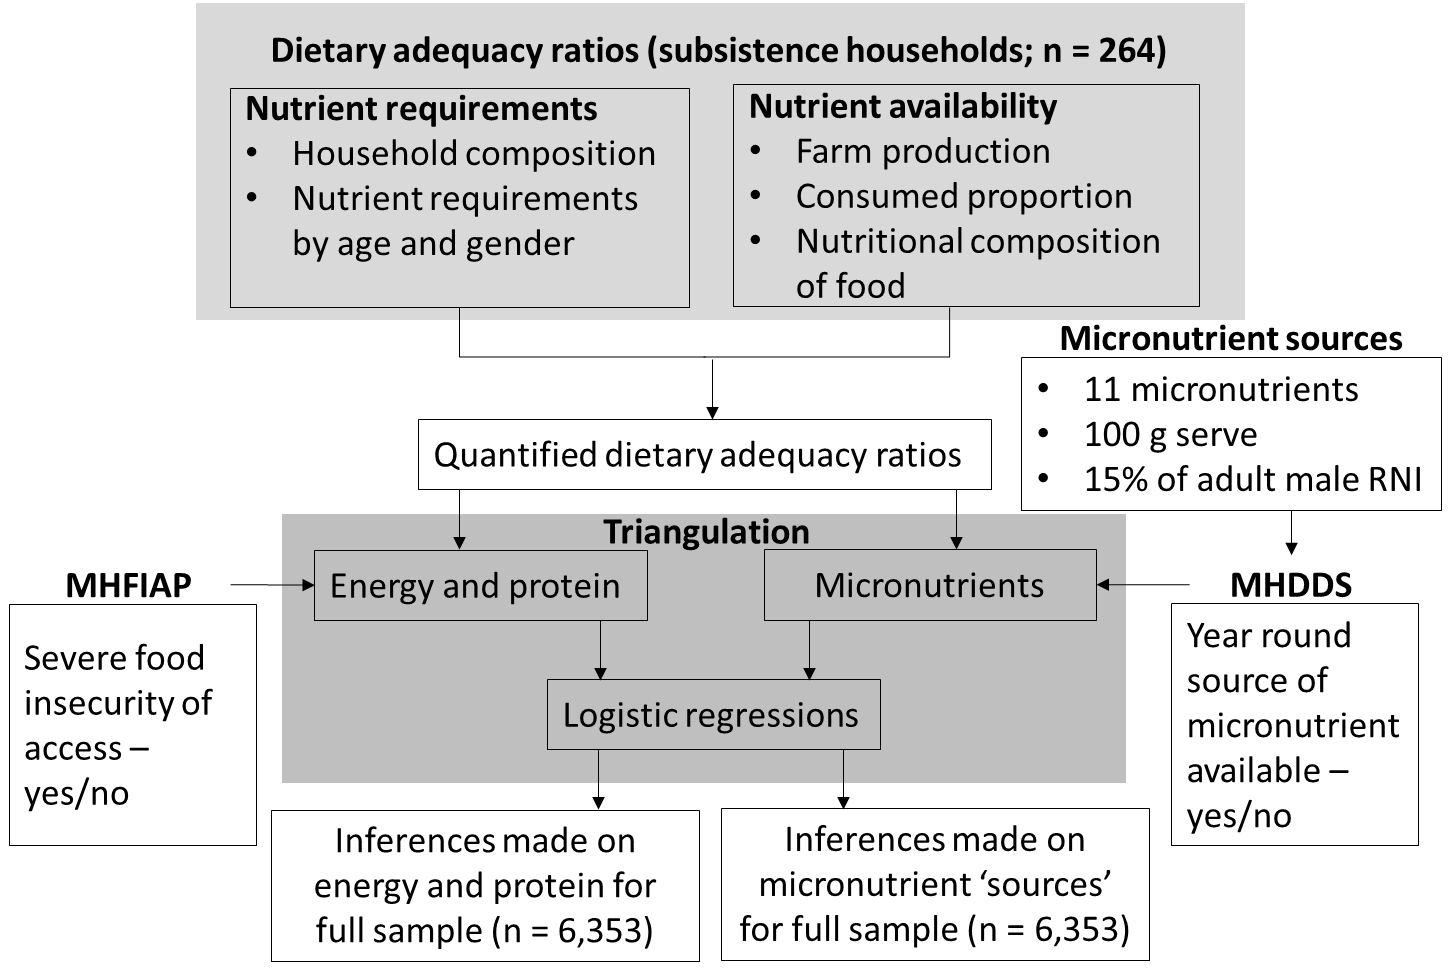
\includegraphics[width=1\textwidth]{figs_06/image1.png}
  \caption{Triangulation of dietary gaps. Dietary adequacy ratios are quantified as the difference between household nutrient requirements and nutrient availability. Sources of micronutrients are identified as food categories (MHDD) that contain at least 15\% of a daily adult male's Recommended Nutrient Intake (RNI). Micronutrient sources and severe food insecurity (MHFIAP) are retained in subsequent analyses if they are associated with their respective quantified gaps}
  \label{fig:06_1}
\end{figure}

The computation of household \textit{nutritional requirements} was based on three established estimates: energy requirements (\citealp{FoodandAgricuturalOrganization2001}), safe level of protein intake (\citealp{WHO2002}) and recommended nutrient intakes (RNI) of micronutrients (\citealp{FAO2004}). Energy requirements were based on gender, an assumed increase in weight/basal metabolic rate (BMR) with age, an assumed moderate physical activity level (PAL value between 1.7 and 1.99) and assumed good health. With these assumptions, the estimated kilocalorie requirement for an adult male between 25 and 50 was 2750 kcal and 2250 kcal for females. Protein intake requirements were based on age and gender categories for children and adolescents and weight for adults. Micronutrient RNIs were based on age and gender categories. The total household requirements for each of these nutrients were then calculated as the sum of requirements by gender and age requirements. Variations in nutritional requirements due to health status, level of activity and interactions between nutrients (e.g. vitamin D promoting calcium absorption) were not accounted for. These limitations may have resulted in underestimates of nutrient requirements for households with poor health status and those that are more active. The resulting quantified dietary adequacy ratios of subsistence households are presented as boxplots in Appendix Figures \ref{fig:A_1} and \ref{fig:A_2}.

Household \textit{nutrient availability} was computed using food consumption volumes, which were estimated using farmer reported details of crop and animal-sourced food production, and their estimated proportion consumed. Meat yield from farm slaughtered animals was estimated based on approximate live weights and carcass composition; all households were assumed to consume liver from the animals that they had slaughtered -- based on dietary preferences for liver and the need to maximise carcass utilisation. Milk yield (minus suckling) was estimated based on farmer estimates of average daily litres on a seasonal basis (flush and lean), with an assumed lactation length of 270 days. The \textit{nutrient availability} of farm-sourced foods was derived from food composition tables specific to Tanzania (n$_{\mathrm{food items}}$ = 62; \citealp{Lukmanji2008}) and supplemented with region-specific values (e.g. fonio millet in West Africa; \citealp{FAO2012}) and USDA food composition tables where necessary (n$_{\mathrm{food items}}$ = 34; \citealp{USDepartmentofAgricultureUSDA2017}). Zinc and iron content was adjusted based on an estimated high dietary phytate to zinc supply ratio (molar ratio {\textgreater} 20 in SSA; \citealp{Joy2014}; defined as high by \citealp{Brown2001}) and the common practice of fermenting cereals (i.e. reducing phytate content, resulting in improved bioavailability; \citealp{Nout2009}). Thus, the bioavailability of zinc was assumed to be `moderate', and a 10\% bioavailability was assumed for iron -- which was held constant across households. The inedible proportions of food items were removed from the nutrient estimate calculations based on United States Department of Agriculture (USDA) proportion values. Modelling was focused on the total availability of nutrients and so did not factor in discarded edible portions (food waste), nor food transformations (e.g. flour and oil).

The association was then assessed between household dietary adequacy ratios and dietary gaps identified through the MHDD and MHFIAP indicators. Severe food insecurity-- as identified in the MHFIAP indicator -- was considered as a proxy for energy and protein adequacy ratios. Gaps in micronutrient `sources' -- as identified through the MHDD indicator -- was compared with micronutrient adequacy ratios. To assess whether households had year-round daily sources of individual micronutrients, we first identified the micronutrients associated with each MHDD food category. A `source' food category of a given micronutrient was defined by having an average availability of at least 15\% of the daily RNI for an adult male per 100 g serve (\citealp{FAO1997}). The average availability per MHDD category was based on the weighted average nutrient composition of farm production (based on sampled households), on a country and (if data limitations required) a regional basis (i.e. East, central and West Africa). As an exception, dairy was assumed to be a source of calcium, with a 100 g serve estimated to meet 12\% of an adult male's daily requirements. In East Africa, for example, three food categories in the MHDD indicator are sources of five or more micronutrients: nuts and seeds; meat, fish poultry; and vitamin A rich vegetables (refer to Appendix Table \ref{tab:C_4} and Appendix Table \ref{tab:C_5}). In contrast, dairy and eggs only provided a limited number of micronutrients but were important sources of those that were less common, namely: calcium (dairy), vitamin A (eggs) and vitamin B12. We assessed whether households had at least one source in both the flush period and lean period and if so, the household was categorised as having a year-round source of that particular micronutrient; if not, they had a dietary gap for that micronutrient.

The statistical associations between quantified adequacy ratios and dietary gaps identified through indicators (gaps in MHDD `sources'; MHFIAP -- severely food insecure) were assessed using logistic regressions for subsistence households only. In this specification, a binary dependent variable (availability of nutrient source through MHDD/HFIAP indicators -- yes/no) was modelled with the corresponding adequacy ratio as the independent variable. Logistic regression was used in favour of alternative statistical approaches so that our decision rule on whether to include/exclude a nutrient in further analysis could incorporate the direction of association (expected to be positive) as well as the statistical significance of the association (expected to have a p-value of less than 0.05).

%Univariate post hoc regression outputs are summarised as coefficient and the probability ... t/z
\subsection{Associations between dietary gaps and livelihood characteristics}

The prevalence of dietary gaps were weighted based on population estimates of the administrative unit that the households were sampled to represent. Population estimates of the year 2015 were extracted from the `gridded population of the world' dataset (version 4; CIESIN, 2017) -- masking out densely populated areas (>1000 people per km$^2$). Observations were then weighted based on the average population density in the administrative unit (persons per km$^2$), relative to other administrative units -- such that each household within an administrative boundary was weighted equally and relative to other administrative boundaries. The weights of studies that only sampled livestock keeping households were adjusted, assuming that they represent 50\% of the rural population. The sum of weights equated to the sample size.

We model associations between nutrient gaps and household composition, farm production mix, market participation and income. Agroecological zone (AEZ) was also included as fixed effects in the regression models to control for the effects of differences between semi-arid locations (Length of growing period; LGP 75 -- 180 days) and humid/sub-humid locations (LGP {\textgreater} 181 days). We incorporated random effects on the intercept from villages nested within projects in our models. We used negative binomial regressions with mixed-effects to model overdispersed count variables (MHDD) and logistic regressions with mixed-effects to model whether households were severely food insecure (of access) or not and whether households have a gap in sources of micronutrients.

To further explore modelled associations, we developed a farm typology based on the composition of farm production -- which influences both cash availability and diversity of own-farm food availability (\citealp{Headey2018}; \citealp{Jones2016}). Farms were classified as `specialised cropping' if they reported two or fewer crop species as being important for their livelihood or sourced two or fewer plant-based food categories (e.g. `legumes' or `leafy vegetables') from their farm; farms with three or more crop species/plant-based categories were classified as having `diverse cultivation'. Livestock holdings (animals under the care of the household) were represented as Tropical Livestock Units (TLU), and households with over 1.5 TLUs (the equivalent of one head of cattle -- 1 TLU, one sow -- 0.3 TLU and five chickens -- 0.04 TLU) were categorised as having a livestock product (meat, milk or eggs) component to their farm, in combination with their cropping activities. This threshold was set marginally higher than one TLU to reduce instances of false positive classifications of households keeping an ox or donkey (0.8 TLU) for draught power purposes. We identified four distinct farm types: `Specialised cropping', `Diverse cropping', `Specialised cropping and livestock', and `Diverse cropping and livestock'. We use this farm typology to characterise channels of food access and to explore the prevalence of food insecurity and dietary gaps (Appendix Table \ref{tab:C_8} provides a regional breakdown of farm types.

Differences between farm types were modelled using mixed-effects linear and logistic regressions, with random effects on the intercept from villages nested within projects. Dependent variables of these models included farm-household characteristics, consumption behaviour and dietary gaps. The independent variable in these models was either farm type or an aggregation of farm types (e.g. livestock keeping). All regression models were estimated using a hybrid Monte-Carlo Markov Chain (MCMC) method, implemented in R using the `BRMS' package (v 1.0.1; \citealp{BuerknerP2016}). Weakly informative priors (Student's t-distribution with df = 5) were used, allowing extreme values but maintaining an expectation of minimal association (i.e. central tendency near zero). The posterior distributions were analysed and if 95\% of the density was above or below zero then it was considered to be significantly associated. Models were based on a core set of household and farm variables, with interactions tested additively. All regressions were weighted by population density -- minimising bias in generalisations to the sampled locations.


%Differences between farm types were modelled using mixed-effects linear and logistic regressions, with random effects on the intercept from villages nested within projects. Dependent variables of these models included farm-household characteristics, consumption behaviour and dietary gaps. The independent variable in these models was either farm type or an aggregation of farm types (e.g. livestock keeping). All linear and negative binomial regressions were performed using the lme4 package in R (\citealp{BatesD2017}). Linear regressions with non-parametric residuals were re-run with cuberoot transformed dependent variables. The statistical significance of fixed effects in linear regressions were assessed using the F-test with Kenward-Roger approximation (\citealp{Kenward1997}), comparing models additively from the intercept only model. All logistic regressions were performed with the glmmPQL function from the MASS package in R (\citealp{Venables2002}), which includes an overdispersion parameter to model the dependence between accumulated binary observations (\citealp{Breslow1993}). The statistical significance of fixed effects in the generalised linear regressions were assessed using the wald test using the aod package in R (\citealp{Lesnoff2012}).


\section{Results}

\subsection{Triangulation to identify energy, protein and micronutrient gaps}

Only 7 of the 11 micronutrients met our triangulation decision rules of statistical significance, a positive association (Table \ref{tab:06_1}). Thus, the nutrients included in the remainder of the results were limited to calcium, iron, thiamine, riboflavin, niacin, vitamin B6 and vitamin B12. Severe food insecurity (of access) in the lean period was associated with year-round energy and protein sufficiency and thus retained as a proxy to these dietary gaps.


\begin{table}[H]
  \captionsetup{singlelinecheck = false, justification=justified}
  \caption{
  Associations between quantified adequacy ratios and dietary gaps identified through indicators for subsistence households (n = 264). Nutritional elements with an inconsistency were excluded from further analyses (Logistic regression outputs -- beta coefficent estimate, standard error and statistical significance)
  }
  \label{tab:06_1}
  \small
\begin{tabular}{L{3cm} C{2.5cm} C{2cm} C{2cm}}
  %{
%p{\dimexpr 0.21\linewidth-2\tabcolsep}
%p{\dimexpr 0.26\linewidth-2\tabcolsep}
%p{\dimexpr 0.26\linewidth-2\tabcolsep}
%p{\dimexpr 0.26\linewidth-2\tabcolsep}}
\toprule
Nutrient & Estimate (SE) & Significance & Retained \\
\midrule
Energy & 1.00 (0.42) & * & x \\
Protein & 0.94 (0.40) & * & x \\
Calcium (Ca) & 2.78 (0.75) & * & x \\
Iron (Fe) & 0.84 (0.40) & * & x \\
Zinc (Zn) & 0.32 (0.41) & & \\
Vitamin A & 0.92 (0.46) & & \\
Thiamine & 0.96 (0.42) & * & x \\
Riboflavin & 0.95 (0.46) & * & x \\
Niacin & 0.94 (0.42) & * & x \\
Vitamin B6 & 0.80 (0.43) & * & x \\
Folate & -0.40 (0.40) & & \\
Vitamin B12 & 2.30 (0.57) & * & x \\
Vitamin C & -0.85 (0.54) & & \\
\bottomrule
\end{tabular}
\footnotesize
\raggedright
%\caption*{
\\
95\% CI does not cross zero\\
x = triangulation decision rules have been met
\end{table}



\subsection{Prevalence of severe food insecurity of access and dietary gaps}

Severe food insecurity (of access) was widespread across the surveyed households (\textit{n =} 6,353). In the lean period as many as 40\% of households were classified as severely food insecure according to the food access assessment with the HFIAP indicator. For micronutrients, 68\% of households did not have a year-round daily source of calcium, 38\% lacked a daily source of iron, 37\% lacked a daily source of thiamine, 51\% lacked a daily source of riboflavin, 44\% lacked a daily source of niacin, 35\% lacked a source of vitamin B6 and 65\% lacked a daily source of vitamin B12 (Table \ref{tab:06_2}).


\begin{table}[H]
  \setlength\dashlinedash{0.2pt}
  \setlength\dashlinegap{1.5pt}
  \setlength\arrayrulewidth{0.3pt}

  \captionsetup{singlelinecheck = false, justification=justified}
  \caption{Prevalence of dietary gaps weighted by population (n= 6,353; \% of weighted sample)}
  \label{tab:06_2}
  \small
\begin{tabular}{L{4.5cm} L{3cm} C{2.5cm}}
  %{\textwidth}{
%p{\dimexpr 0.44\linewidth-2\tabcolsep}
%p{\dimexpr 0.37\linewidth-2\tabcolsep}
%p{\dimexpr 0.19\linewidth-2\tabcolsep}}
\toprule
Proxy for dietary gap & Dietary requirement & Prevalence \\
\midrule
Severe food insecurity & Energy and protein & 40 \\
\arrayrulecolor{black!30}\midrule
%\hdashline
Source category accessed & Calcium (Ca) & 68 \\
daily throughout the year & Iron (Fe) & 38 \\
 & Thiamine (B1) & 37 \\
 & Riboflavin (B2) & 51 \\
 & Niacin (B3) & 44 \\
 & Vitamin B6 & 35 \\
 & Vitamin B12 & 65 \\
 \arrayrulecolor{black}\bottomrule
\end{tabular}
\end{table}

There are several factors associated with MHFIAP, MHDD and micronutrient sourcing (Table \ref{tab:06_3}). Regression results show that the number of household inhabitants was positively associated with diet diversity in the flush and lean periods as well as vitamin B12. The number of household inhabitants was also positively associated with the availability of year-round sources of thiamine and riboflavin in humid/subhumid zones. Female headed households were negatively associated with food security of access in the lean period and were less likely to have year-round sources of calcium. Having children under the age of 10 in the household was negatively associated with food security of access and diet diversity in the lean period, and negatively associated with having year-round sources of calcium and vitamin B12. These results suggest that there are household compositions with greater vulnerability to chronic and hidden hunger, which differs by AEZ in the instance of the number of household inhabitants.

Land cultivated was positively associated with having sources of calcium, iron, thiamine, and vitamin B6. However, in humid/subhumid zones land cultivated was negatively associated with access to sources of calcium. Livestock holdings were negatively associated with food security of access and diet diversity in the lean period. However, the association with diet diversity in the lean period was the weakest of all significant coefficients (Appendix Table \ref{tab:C_7}). Livestock holdings were also positively associated with diet diversity in the flush period (Figure \ref{fig:06_2}) and positively associated with the availability of sources for all micronutrients in both semi-arid and humid/sub-humid zones.

Market participation was positively associated with food security of access, diet diversity in both the flush and lean periods and positively associated with the availability of calcium, thiamine, riboflavin, vitamin B6 and vitamin B12. Off-farm income was positively associated with food security of access, diet diversity in both periods, as well as iron, thiamine, riboflavin, niacin, vitamin B6 and vitamin B12. Gross income was positively associated with food security of access, diet diversity in the flush and lean periods, and positively associated with the availability of sources of riboflavin and vitamin B12.

Crop production diversity was positively associated with food security of access in semi-arid zones, diet diversity in the flush and lean periods. In humid/subhumid zones, crop production diversity was negatively associated with food security of access. Crop production diversity was positively associated with the availability of iron, thiamine and niacin and negatively associated with calcium. The diversity of livestock products produced by a household was positively associated with food security of access, diet diversity in the lean period as well as being positively associated with calcium and vitamin B12. Livestock production diversity was negatively associated with iron, thiamine, and vitamin B6.

These results suggest that associations between diets and farm-household characteristics differ between AEZs. These differences between AEZs were most substantial for market participation and crop production diversity (full regression outputs shown in Appendix Table \ref{tab:C_7} and additional marginal effects presented in Appendix Figure \ref{fig:A_3}).


\begin{sidewaystable}
\centering
\captionsetup{singlelinecheck = false, justification=justified}
  \caption{
  Associations between nutrition (dependent variables in columns) and livelihood characteristics and agroecological zone (AEZ). Mixed-effects logistic\textasciicircum{} and negative binomial$^{\dag}$ regressions, displaying the direction of association for statistically significant explanatory variables (n = 6,353)
  }
  \label{tab:06_3}
  \small
  \centering
\begin{tabularx}{\textwidth}{
p{\dimexpr 0.29\linewidth-2\tabcolsep}
p{\dimexpr 0.08\linewidth-2\tabcolsep}
p{\dimexpr 0.07\linewidth-2\tabcolsep}
p{\dimexpr 0.08\linewidth-2\tabcolsep}
p{\dimexpr 0.04\linewidth-2\tabcolsep}
p{\dimexpr 0.04\linewidth-2\tabcolsep}
p{\dimexpr 0.08\linewidth-2\tabcolsep}
p{\dimexpr 0.09\linewidth-2\tabcolsep}
p{\dimexpr 0.06\linewidth-2\tabcolsep}
p{\dimexpr 0.07\linewidth-2\tabcolsep}
p{\dimexpr 0.07\linewidth-2\tabcolsep}}
\toprule
 & MHFIAP\textasciicircum{} & HDD flush period$^{\dag}$ & HDD lean period$^{\dag}$ & Ca\textasciicircum{} & Fe\textasciicircum{} & Thiamine\textasciicircum{} & Riboflavin\textasciicircum{} & Niacin\textasciicircum{} & Vitamin B6\textasciicircum{} & Vitamin B12\textasciicircum{} \\
 \midrule
Intercept &  & + &  & - & & & & & & - \\
Household inhabitants (adulteq.) &  & + & + & & & & & & & + \\
Female household head (yes) & - &  &  & - & & & & & & \\
Children under 10 (yes) & - &  & - & - & & & & & & \\
\arrayrulecolor{black!30}\midrule
Land cultivated (ha) &  &  &  & + & + & + & & & + & \\
Livestock holdings (TLU) & - & + & - & + & + & + & + & + & + & + \\
Market participation (\% kcal sold) & + & + & + & + & & + & + & & + & + \\
Off-farm income (yes) & + & + & + & & + & + & + & + & + & + \\
Gross income (PPP) & + & + & + & + & & & + & & & + \\
Crop production diversity${\ddag}$ & + &  & + & - & + & + & & + & & \\
Livestock product diversity${\ddag}$ & + & + & + & + & - & - & & & - & + \\
\arrayrulecolor{black!30}\midrule
AEZ (sub-)humid{\S} & + & + &  & + & - & - & + & & - & + \\
Household members:AEZ{\S} &  & + &  & & & + & + & & & \\
Land cultivated:AEZ{\S} &  &  &  & - & + & & & & & \\
Livestock holdings:AEZ{\S} &  &  &  & & + & & & & & \\
Market participation:AEZ{\S} & - &  &  & & & & & & & - \\
Crop production diversity:AEZ{\S} &  &  & + & & & & & + & + & \\
\arrayrulecolor{black}\bottomrule
\end{tabularx}
\footnotesize
\raggedright
%\caption*{
$^{\ddag}$Number of crop/livestock MHDD categories produced\\
$^{\S}$AEZ reference category = semi-arid\\
+ Statistically significant positive association; - statistically significant negative association

\end{sidewaystable}

\newpage



\begin{figure}[H]
  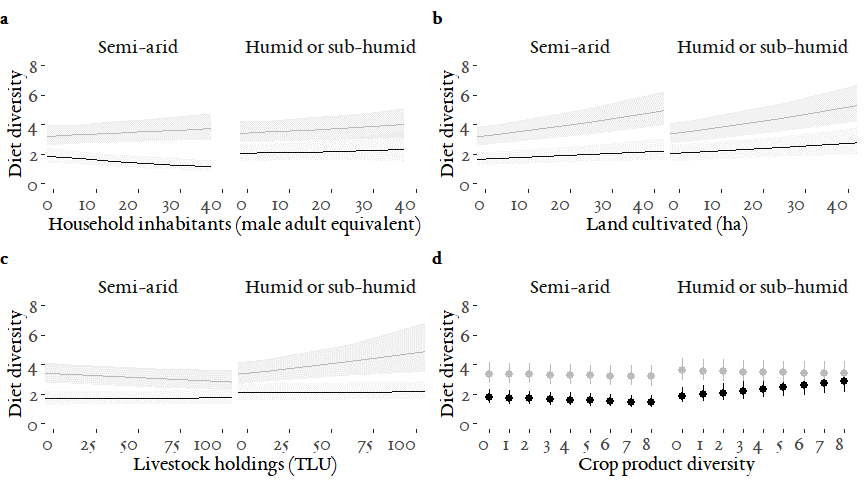
\includegraphics[width=1\textwidth]{figs_06/image2.png}
  \captionsetup{singlelinecheck = false, justification=justified}
  \caption{Predicted associations between MHDD and a) household inhabitants (adult eq), b) land cultivated, c) livestock holdings (Tropical Livestock Units), d) crop product diversity in the flush (grey line/point) and lean (black line/point) periods by agroecological zone}
  \label{fig:06_2}
\end{figure}

\subsection{Channel of food access and dietary gaps by farm type}

Households with a livestock component tended to have more people in the household, larger land area cultivated, better `progress out of poverty' and -- naturally -- more livestock (mixed-effects linear regressions; 95\% CI > 0; Appendix Table \ref{tab:C_11}). `Diverse cropping' and `Diverse cropping and livestock' households tended to have greater market participation than their specialised counterparts (mixed-effects linear regression; 95\% CI > 0; Appendix Table \ref{tab:C_12}). Farm types with a livestock component had significantly higher MHDD scores in the flush and lean periods compared to other farm types (Table \ref{tab:06_4}; mixed-effects linear regression; 95\% CI > 0; Appendix Table \ref{tab:C_11}). As expected, all farm types had higher median MHDD scores in the flush period, compared to the lean period.


\begin{table}[H]
  \captionsetup{singlelinecheck = false, justification=justified} %left justify caption
  \caption{
  Summary of resources, income and diet diversity of sampled households by farm type (number, proportion and median-IQR)
  }
  \label{tab:06_4}
  \small
\begin{tabularx}{\textwidth}{@{}lYYYY@{}}
%  {
%p{\dimexpr 0.29\linewidth-2\tabcolsep}
%p{\dimexpr 0.14\linewidth-2\tabcolsep}
%p{\dimexpr 0.15\linewidth-2\tabcolsep}
%p{\dimexpr 0.14\linewidth-2\tabcolsep}
%p{\dimexpr 0.15\linewidth-2\tabcolsep}
%p{\dimexpr 0.15\linewidth-2\tabcolsep}}
\toprule
 & Specialised cropping & Diverse cropping & Specialised cropping \& livestock & Diverse cropping \& livestock\\
 \midrule
n & 719 & 1596 & 1085 & 2943\\
Subsistence households (\%) & 4 & 4 & 5 & 4 \\
AEZ (Sub-)humid (\%) & 52 & 61 & 31 & 44 \\
Smallholders (\% ${\leq}$2 ha) & 44 & 39 & 34 & 32 \\
Mixed crop-livestock (\%) & 3 & 4 & 17 & 25 \\
Household members (adult equivalents) & 4.5 (3.4) & 4.9 (3.7) & 5.9 (4.2) & 5.9 (3.8)  \\
\arrayrulecolor{black!30}\midrule
Land cultivated (ha) & 1.06 (1.39) & 1.42 (1.62) & 2 (3.05) & 1.82 (3.19) \\
Livestock holdings (TLUs) & 0.2 (0.7) & 0.3 (0.8) & 7.6 (24.1) & 7.0 (10.3)  \\
Off-farm income (PPP$^{-1}$ year) & 0 (0) & 0 (30) & 0 (0) & 0 (150)  \\
Progress out of Poverty Index score & 33 (26) & 29 (40) & 41 (23) & 45 (26)  \\
Market participation (proportion kcal sold) & 0.03 (0.50) & 0.25 (0.55) & 0.05 (0.44) & 0.25 (0.49) \\
Crop income (PPP$^{-1}$ year) & 0 (210) & 86 (507) & 0 (47) & 65 (629)  \\
Live animal (PPP$^{-1}$ year) & 0 (0) & 0 (11) & 1 (128) & 3 (275)  \\
Livestock product income (PPP$^{-1}$ year) & 0 (9) & 0 (19) & 3 (195) & 69 (480)  \\
\arrayrulecolor{black!30}\midrule
Daily diet diversity -- flush period & 2 (2) & 4 (4) & 3 (2) & 4 (3) \\
Daily diet diversity -- lean period & 1 (2) & 1 (3) & 2 (2) & 2 (3)  \\
\arrayrulecolor{black}\bottomrule
\end{tabularx}
\footnotesize
\raggedright
%\caption*{

\end{table}

\vspace{-0.5cm}

The channel of accessing MHDD food categories differed by farm type. In Figure \ref{fig:06_3} two channels of access -- farm sourced and purchased -- and total diet diversity for the four farm types are presented for the lean period (equivalent results for the flush period are presented in Appendix Figure \ref{fig:A_4}).

In Figure \ref{fig:06_3}, the probability density function of the count of household diet diversity (MHDD) categories is presented as a black line on the lower half of each facet. The line indicates the probability that a household in a given farm type consumes a given number of categories (1-10). Each facet also presents the proportion of households that consume certain categories for a given count of MHDD. For example, in the top right-hand facet showing `Specialised cropping' and `total', the second pillar shows households with only two MHDD food categories, where the most common daily sourced food category was `grains, roots, tubers and plantains', followed by `leafy vegetables', `other vegetables' and then `legumes'. In contrast, since the far-right pillar shows households which consume all 10 food categories, the proportions of each are equal. {Figure \ref{fig:06_4}} allows comparison between farm types for a specific channel and within farm types, between channels. Inference from this figure is focused on the central mass of the probability density function -- generally between 1 and 5 MHDD categories.

\begin{figure}[H]
  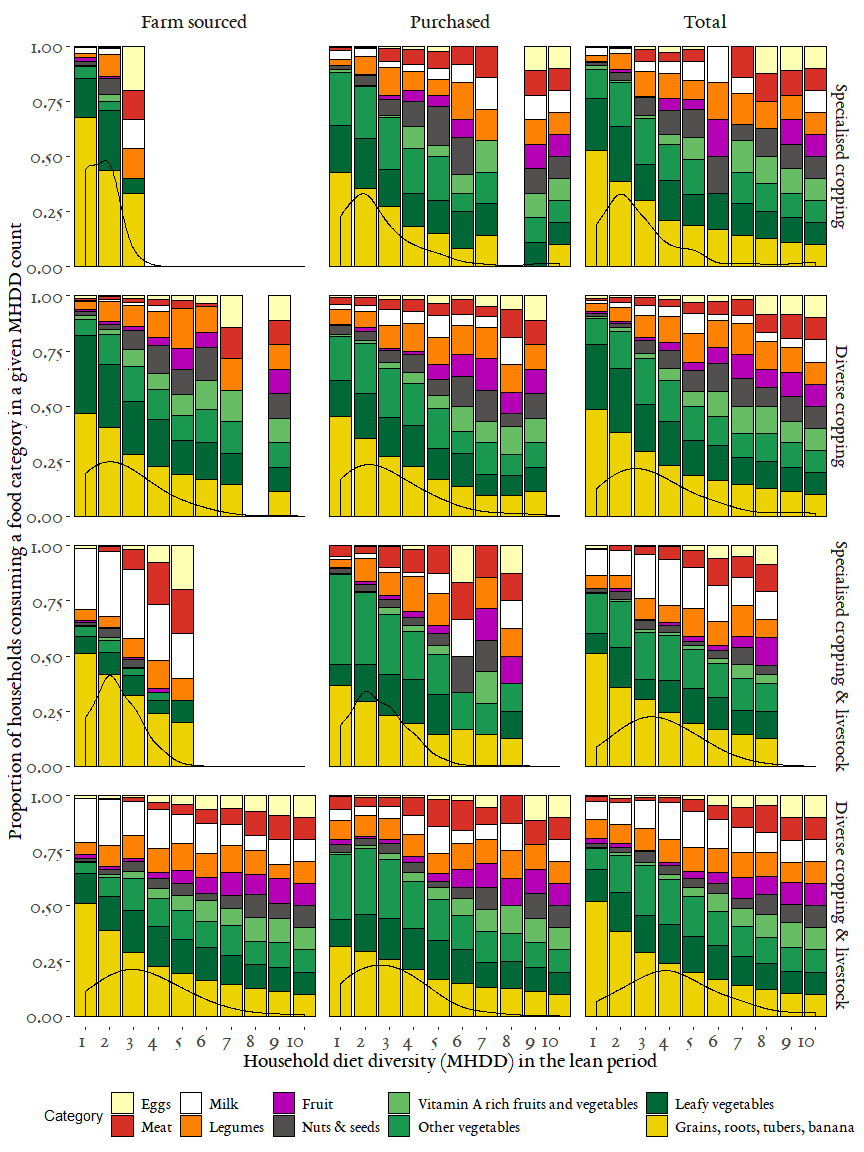
\includegraphics[width=1\textwidth]{figs_06/image3.png}
    \captionsetup{singlelinecheck = false, justification=justified}
  \caption{Diet diversity: density and proportion of sampled households (n=6,353) consuming specific food categories by farm type, channel of access and total diet diversity in the lean period. The distribution (probability density function) of diet diversity for each period is represented as a black line on the lower half of each figure facet. Food categories are represented by different colours, showing the proportion of households consuming each category at specific diet diversity levels}
  \label{fig:06_3}
\end{figure}

At the aggregate level, farm types with a substantial livestock component consume more livestock products -- milk, meat and eggs -- in both flush and lean periods (mixed-effects logistic regressions; 95\% CI > 0 for all animal source foods; Appendix Table \ref{tab:C_11}). In the lean period, 50\% of households with a livestock component to their farm consumed dairy products compared to less than 17\% of crop-oriented households. In Figure \ref{fig:06_3}, it is evident that dairy products are predominantly accessed through the farm channel and are sometimes the only daily sourced food category. Meat consumption -- a source of vitamin B12 among several other micronutrients -- in the lean period was marginally higher in households with a livestock component (38\% compared to 28\% of crop-based households). Meat was most often purchased, particularly in the flush period -- irrespective of farm type. Daily egg consumption -- also a source of vitamin B12 and riboflavin -- was less common, but consistently higher in households with a livestock component (results not tabulated elsewhere).

A greater proportion of households with a diverse cropping component to their farm tended to source plant-based food categories in the flush period -- except `nuts and seeds' and `grains, roots, tubers and banana' (mixed-effects logistic regressions;  95\% CI > 0 for all plant-based categories; Appendix Table \ref{tab:C_12}). In the lean period, when compared to other farm types, a smaller proportion of households in the `Specialised cropping' farm type sourced `legumes', `fruit', `vitamin A rich fruits and vegetables', and `other vegetables'.


The prevalence of severe food insecurity (of access) was not independent of farm type in both humid/sub-humid and semi-arid agroecological zones (Table \ref{tab:06_5}).

\begin{table}[H]
  \captionsetup{singlelinecheck = false, justification=justified}
  \caption{
  Associations between severe food insecurity, farm type and agroecological zone (AEZ). Mixed-effects logistic regression.
  }
  \label{tab:06_5}
  \small
\begin{tabular}{L{8cm} C{2.5cm} C{2cm} C{2cm}}

\toprule
 & estimate (SE) & Significance \\
\midrule
Intercept & -0.51 (0.91) &  \\
Diverse cropping$^\dag$ & -0.32 (0.16) & * \\
Specialised cropping \& livestock$^\dag$ & -0.92 (0.16) & * \\
Diverse cropping \& livestock$^\dag$ & -0.41 (0.17) & * \\
AEZ$^\ddag$ & 0.05 (0.12) & \\
\bottomrule
\end{tabular}
\footnotesize
\raggedright
%\caption*{
\\
95\% CI does not cross zero\\
$^\dag$Reference category is `Specialised cropping' \\
$^\ddag$Reference category is semi-arid
\end{table}

Specialised cropping households tended to have a higher prevalence of severe food insecurity -- when compared with all other farm types (Table \ref{tab:06_5}). In humid/sub-humid AEZs, households with `Diverse cropping \& livestock' had a lower prevalence of severe food insecurity and gaps in all micronutrients, when compared to other farm types (mixed-effects logistic regressions; 95\% CI > 0; Appendix Table \ref{tab:C_13_2}; Figure \ref{fig:06_4} and Appendix Figure \ref{fig:A_5}). In semi-arid zones, the difference between farm types was more distinct, where households with a livestock component to their farm had a significantly lower prevalence of calcium and vitamin B12 (mixed-effects logistic regressions; 95\% CI > 0 for MHFIAP and all micronutrients; Appendix Table \ref{tab:C_13_3}).

\begin{figure}[H]
  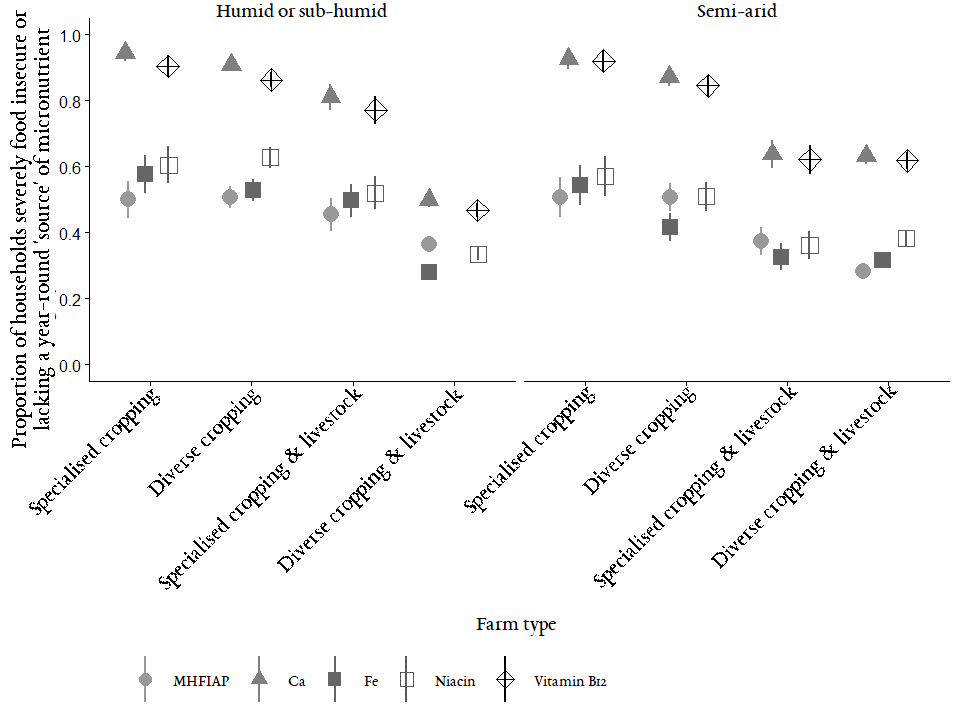
\includegraphics[width=1\textwidth]{figs_06/image4_weighted2.png}
  \captionsetup{singlelinecheck = false, justification=justified}
  \caption{Proportion of households (n = 6,353 weighted by population) with insecure access to food (MHFIAP) or no `source' of calcium, iron, niacin, or vitamin B12 by farm type and agroecological zone. A 95\% confidence interval is represented by vertical lines}
  \label{fig:06_4}
\end{figure}

\section{Discussion}

\subsection{Food insecurity and dietary gap prevalence}

The aim of this study was to combine diet diversity and food (in)security indicators with household-farm characteristics to estimate prevalence of dietary gaps and to understand their associations with rural livelihoods and food sourcing behaviour throughout the year. In addition to generating key information on food security of access and dietary diversity over the course of the year for a wide range of contrasting systems in sub-Saharan Africa, our approach also allowed us to quantify dietary gaps for six important micronutrients (Table \ref{tab:06_2}): calcium, iron, thiamine, riboflavin, niacin, vitamin B6 and vitamin B12.

The prevalence of dietary gaps in this study are comparable to previous studies, despite the substantial differences in target populations and sampling procedures. An estimated 40\% of sampled households were severely food insecure in their access to food; this is higher than reported by the FAO using the Food Insecurity Experience Scale (FIES; Appendix Table \ref{tab:C_10} provides a comparison of the questions asked) -- with an estimated 34\% of the SSA population being severely food insecure in 2017 (\citealp{FAO2018}). An estimated 68\% of households did not source calcium-rich food categories on a daily basis, which is between deficiency prevalence estimates derived from \citet[calculated as the inverse weighted average of the probability of adequacy -- Appendix Table \ref{tab:C_11}; calcium deficiency prevalence was 91\% of sampled women in Burkina faso, Mali and Uganda]{Martin-Prevel2015} and \citet[54\% of individuals in Africa]{Joy2014}. Our estimates of gaps in iron availability (38\% of households) are lower than the deficiency prevalence estimates in \citet[78\%]{Martin-Prevel2015}, but within the range of estimates in \citet[whose estimates range from 5\% assuming low bioavailability (10\% available), to 43\% for very low bio-availability (5\% available)]{Joy2014}. Our estimates for thiamine (37\%), riboflavin (51\%), niacin (44\%) and vitamin B6 (35\%) are comparable to estimates in \citet[thiamine 32\%, riboflavin 56\% and niacin 34\%, vitamin B6 26\%]{Martin-Prevel2015}. Additionally, an estimated 66\% of households did not source vitamin B12 rich food categories on a daily basis, which is more conservative than the deficiency prevalence estimates derived from \citet[93\% of sampled women]{Martin-Prevel2015}.

\subsection{Contextual factors for targeting nutrition-sensitive interventions}

There are several factors associated with food security of access, diet diversity and the daily sourcing of micronutrients. From the perspective of designing nutrition-sensitive agricultural interventions, we discuss a) contextual factors that can improve the targeting of interventions and b) factors that can form the basis of an intervention or be incorporated as a complementary intervention.

The contextual factors identified in this study are either not possible to change through agricultural interventions (AEZ and household composition), or relate to complex farmer/household decisions that are beyond the scope of current public and civil society interventions in SSA (farm scale and farm type). These contextual factors can be used as inputs into the intervention targeting decision-making process, where the aim is to maximise the potential for practice adoption and impact on well-being. On the basis of our results, we expect households with `female heads' and children under 10 years of age to have a higher likelihood of severe food insecurity in the lean period -- supporting the need for programmatic strategies on gender inclusion (\citealp{Mason2015}), as well as focusing on the first 1000 days of life (\citealp{DePee2017}). Similarly, households with small land cultivation areas can be targeted to counteract the tendency of limited access to micronutrient sources (land size has been linked to both chronic and hidden hunger; \citealp{Godecke2018}).

Understanding the existing production systems (farm types) of rural households within and between locations can inform more advanced intervention targeting decisions. For example, an intervening agent (e.g. government, NGO, etc.) may initially target their interventions based on AEZ, farm scale and sub-sector (e.g. dairy), and then in the advanced stages, design and target interventions based on the prevailing farm types. This approach can improve the suitability of interventions to existing conditions (i.e. by enhancement, diversification, or substitution; \citealp{Fiorella2016}) and therefore maximises adoption potential. This contextual factor also provides opportunities to improve the nutrition sensitivity of interventions. Our results show that prevalence rates differ by farm type and AEZ (Figure \ref{fig:06_4}). For example, households without a livestock component had high instances ({\textgreater}80\%) of gaps in calcium and vitamin B12 sources. Intervention packages can be developed to address such dietary gaps, targeting specific farm types in specific AEZs (\citealp{Hetherington2017}; \citealp{Mulmi2017}; \citealp{Hoddinott2012}). This is also reinforced by \citet{Carletto2015}, who review a series of studies showing that a household's agricultural production can directly influence the dietary patterns of household members, where the extent of impact depends on a variety of factors including location, commodities produced, and whether a household keeps livestock for direct consumption.

\subsection{Designing nutrition-sensitive interventions}

There are three factors identified in this study that could be incorporated in nutrition-sensitive agricultural orientated interventions. Increasing farm income (in-part through increasing market participation), improving off-farm employment opportunities (including along the agricultural value-chain; \citealp{Davis2017}) and diversifying production (crops, home garden and livestock products) each had positive effects on food security of access, dietary diversity, and thereby providing sources of micronutrients. These results are in line with the overview presented by \citet[p.~147]{Ruel2018}, stating that `production diversity and livestock ownership are consistently associated with household and dietary diversity and, when measured, with increased intake of essential micronutrients'. There are, however, instances of negative associations with these variables -- such as livestock holdings and diet diversity in the lean period. Extreme increases in income or production diversity (i.e. from the lowest end of the scale to the highest), however, is only predicted to increase diet diversity in the lean period by 1 or 2 food categories (Figure \ref{fig:06_2}). This limitation needs to be taken into account when designing and monitoring nutrition-sensitive interventions. Success may not be measured in leaps in diet diversity, but rather by adding specific food categories (in sufficient frequency and quantity) that provide micronutrient sources that would otherwise be lacking.

\subsection{How do farm types differ in food sourcing behaviour?}

Our results clearly demonstrate that sourcing of food categories was strongly related to farm type (Figure \ref{fig:06_3}). We found that the farm-based route to dietary diversity was extremely important: consumption of specific food groups is strongly linked to what farm households produce on-farm. This is a key finding because a substantial part of households that lacked an aspect of production diversity -- and thereby miss certain avenues in the farm-based route to dietary diversity -- did not choose to supplement their lack of production diversity with an equivalent diversity of purchased food categories. Households with a livestock component to their farm consumed more livestock products -- in-part due to their on-farm availability (also identified by \citealp{Hetherington2017}). Dairy, for example, was predominantly sourced from the farm in the lean period, where 50\% of households with a livestock component to their farm consumed dairy products compared to less than 17\% of crop-oriented households. Similarly, households with a diverse cropping component to their farm sourced a greater diversity of fruit and vegetable food categories (legumes, fruit, vitamin A rich produce, and other vegetables) -- mainly from the farm.

The finding that only a subset of households supplement gaps in production diversity with an equivalent diversity of purchased food categories indicates that extra income does not necessarily translate into food and nutrition security -- particularly for hidden hunger. Rather, dietary choices are -- in part -- driven by the retail environment, resulting in increased consumption of processed and sweetened foods (categorised as `grains, roots, tubers and banana'; `dairy'), increased instances of obesity and a higher burden of disease (\citealp{Demmler2018}; \citealp{GBD2016RiskFactorsCollaborators2017}; \citealp{Popkin2014}). Therefore, interventions aiming at improving dietary diversity through increasing incomes need to accompany their interventions with nutritional education to stimulate more diverse and nutritious purchases (\citealp{Dhanarajan2017}), or by stimulating production to improve local availability (globally, we lack sufficient fruit and vegetables for 22\% of the human population; \citealp{Siegel2014}). Otherwise, our results suggest that income-based interventions are unlikely to be nutrition-sensitive.

\subsection{Methodological considerations}

In this study we identified important associations between agricultural activities and pathways towards food security of access, diverse diets and gaps in micronutrient sources. These results, however, are limited by the means of data collection, the approximations made, the limited scope of analysis and the indicators used.

We used information collected in one-off (i.e. cross-sectional) household surveys, which are prone to non-credible values and reduced measurement precision. In total 1,355 observations (20\%) were removed from the original dataset -- largely due to missing MHDD data, as well as non-credible household or farm characteristics, and enumerator evaluated quality (Appendix Table \ref{tab:C_3}). Surveys were implemented using the same survey design, implimented with multi-stage clustered sampling strategies. The sampled households were more likely to be in lower socio-economic regions of rural SSA and so can not be taken to represent rural SSA as a whole. Population weightings were based on modelled data based on national statistics with variable quality.

The standard recall procedures of our food security indicators were adapted to enumerate both the lean and flush periods -- allowing us to capture the substantial variation of farm household diets throughout the year. This adaptation on the recall procedure, however, means that respondents may need to remember a set of circumstances from up to 11 months prior in order to answer a question -- potentially having a negative impact on measurement precision (\citealp{Beegle2012}).

The triangulation of energy, protein and micronutrients was based on a series of approximations on requirements and availability. These approximations were also based on data with known inaccuracies (\citealp{Joy2014}) and limited geographical representativeness (utilising food composition data from Tanzania and USDA). These challenges also plague more detailed dietary assessments across Africa (\citealp{Vila-real2018}) and will only improve if there are concerted efforts to generate high quality national and regional food composition tables across the continent. The triangulation is also limited by only assessing the dietary gaps in subsistence households; the diets of households that purchase foods may differ substantially in composition and quantity (\citealp{Popkin2014}). This limitation could be supplemented by information from country specific 24 hour recall datasets. Further work in using diet diversity indicators to assess micronutrient availability could also conduct sensitivity analyses to test the robustness of the triangulation procedure and the effect of farm classification on disaggregated diet gap prevalence.

Limiting our scope to the household level automatically limited the depth of the dietary gap analysis. This has consequences for the interpretation of results. For example, having a source of micronutrient as we have quantified in this study will have different implications for small households (likely to result in sufficiency) as opposed to larger households (they may access a micronutrient daily source but it is not enough for all members). Similarly, we naturally encounter the limitation for any household level indicator: it is not always clear whether we can translate household level findings into consequences for individual members of the family, for example: young children (\citealp{Caraher2016}).

In this study, we only assessed a limited set of indicators and associations. Although agriculture is a crucial determinant of food and nutrition security in landholding households, it is important to understand interactions with factors like education, gender, food preparation and sanitation to understand the full nutritional, and health consequences of our findings (in contrast, \citealp{Godecke2018} and \citealp{Ramankutty2018} do show associations with education and sanitation and \citealp{Dzanku2019} shows associations with gender). A substantial number of studies have reported the benefits of food security of access and a diverse diet on intermediary nutrition outcomes, such and child and maternal intake of ``target'' foods and micronutrients. Evidence of impact on nutrition outcomes -- particularly child anthropometry and micronutrient status -- was much more limited (\citealp{Gillespie2017}), stressing the limitations of using indicators like dietary diversity when inferring nutritional consequences (e.g. \citealp{Hetherington2017} showed weak and inconsistent associations between animal-source food consumption and anthropometric measurements).

Despite these inherent limitations of the analyses, we have quantitatively linked farming system characteristics to food and nutrition security indicators across a wide range of different production systems in sub-Saharan Africa. The most novel feature of this approach is that we can better understand how food security of access, diet diversity and micronutrient sourcing is related to the livelihood characteristics of a rural household over the course of a year (e.g. \citealp{Hammond2017225}). There is substantial variation in household diets, clear associations with livelihood characteristics and differences in food sourcing behaviour between farm types. These insights give confidence that simple approaches -- as used in RHOMIS -- can inform interventions at various levels to improve food and nutrition security in the diverse rural communities of SSA.

\section{Acknowledgments}

This research was made possible by several donors (listed in Appendix Table \ref{tab:C_1}). We would like to extend our gratitude to the rural households that participated in this research and the enumerators who guided the conversations.
